\subsection{Fitting a standard GP}

\subsubsection{Model selection}

We have chosen the locally perioduc kernel~\cite[11]{duvenaud2014automatic},
as the function we are fitting is periodic locally but changes
globally. This kernel is the product of a periodic kernel and radial basis function kernel:
\[
  k( \sigma^2, \ell, p ; x, x')
  = \sigma^2
    \exp{\left(-\frac{2 \sin^2{(\pi | x - x' | / p)}}{\ell^2} \right)}
    \exp{\left( -\frac{(x - x')^2}{2 \ell^2} \right)}
\]
It has three parameters:
\begin{itemize}
  \item $\sigma^2$: The output variance.
  \item $\ell$: The lengthscale which determines the length of the \enquote{wiggles}.
  \item $p$: The period of the periodic kernel.
\end{itemize}
%
Our probabilistic model is then:
\begin{align*}
  p(\theta , y | X)
  &=
  \mathcal{N}(0, K(X) + \epsilon I)
  \\
\intertext{where}
  K(X)_{i,j} &= k(\theta ; x_i, x_j)
  \\
  \theta &= (\sigma^2, \ell, p)
\end{align*}

We assume that we know the noise $\epsilon = 0.01$ which we keep fixed,
so the variable parameters are $\theta = (\sigma^2, \ell, p)$.
We justify keeping the noise fixed as is very small,
which would suggest that we are able to sample the underlying function
very precisely, and so we would likely have good idea of what the noise is.

For the variable parameters, we choose relatively uninformed priors
of $\text{LogNormal}(0, 1)$ for each parameter, meaning we don't
assume much prior knowledge of the function other than the fact that
it is locally periodic and has low noise.
The reason the priors are log-normal rather than just normal
is that we want to ensure our parameters are positive.

\subsubsection{Computing the MAP estimate}

For computing the maximum a-posteriori estimate $\theta^\ast$
we used gradient descent via Pyro's autoguide and the Adam optimizer.
It was trained over 2000 iterations and with a learning rate of $0.02$.
The learned parameters were
$\theta^\ast = (\sigma^2 \approx 2.19, \ell \approx 0.75, p \approx 0.67)$.
The GP prediction and 95\% confidence interval of the predictions
is shown in~\cref{gp:map:pred},
and the log-likelihood of the test data is $\sim -12.99$.

\begin{figure}[htbp]
  \centering
  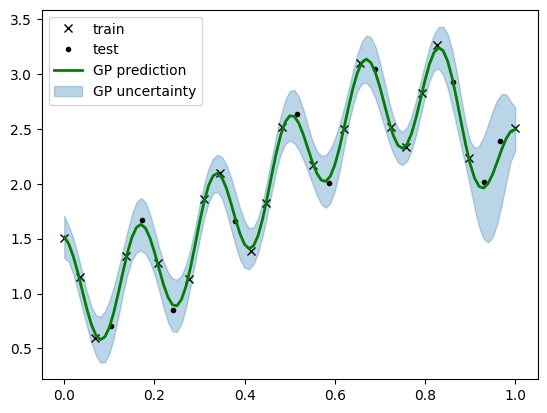
\includegraphics[width=0.6\textwidth]{./figures/map_pred.png}
  \caption{
    Prediction using MAP.
  }
  \label{gp:map:pred}
\end{figure}

\subsubsection{Sampling from the posterior with NUTS}

The hyperparameters for sampling with NUTS is as follows:
\begin{itemize}
  \item Warmup steps: 2000
  \item \# of chains: 4
\end{itemize}
These were chosen via experimentation and observing the diagnostics
from Arviz. The sample trace and posteriors are shown in~\cref{gp:nuts:trace} and \cref{gp:nuts:post} resp.
As can be seen from the trace, the four chains mostly converged to the same parameters,
except for the length where there is some divergence.
From the posterior samples we see that the distributions of the parameters
are (for the most part) unimodal, which is a good sign.

The predictions using a random sample from the posterior is shown in~\cref{gp:nuts:pred}.
The log-likelihoods of the test data is shown in~\cref{gp:nuts:ll}.
The mean and variance of the log-likelihoods is $-11.82$ and $1.76$ resp.

\begin{figure}[htbp]
  \centering
  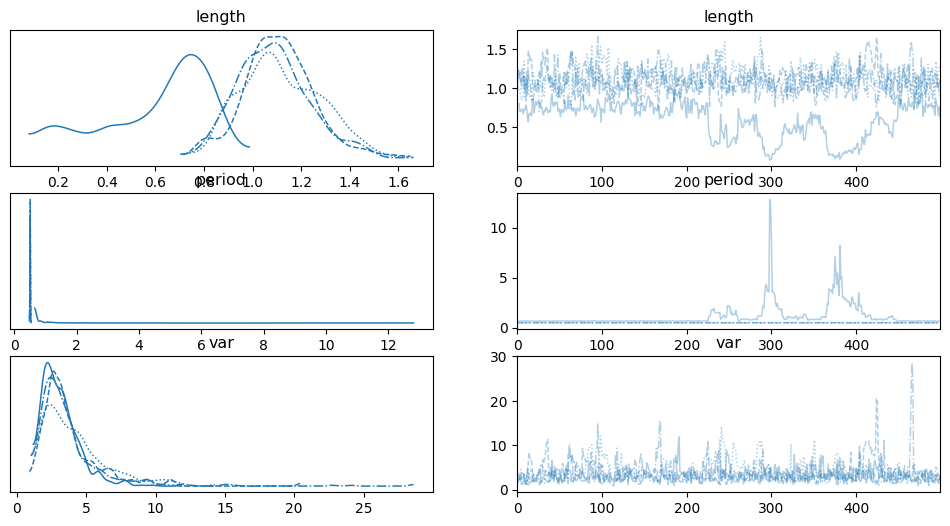
\includegraphics[width=1\textwidth]{./figures/nuts_trace.png}
  \caption{
    Sample trace for the 4 different chains over model parameters.
  }
  \label{gp:nuts:trace}
\end{figure}
\begin{figure}[htbp]
  \centering
  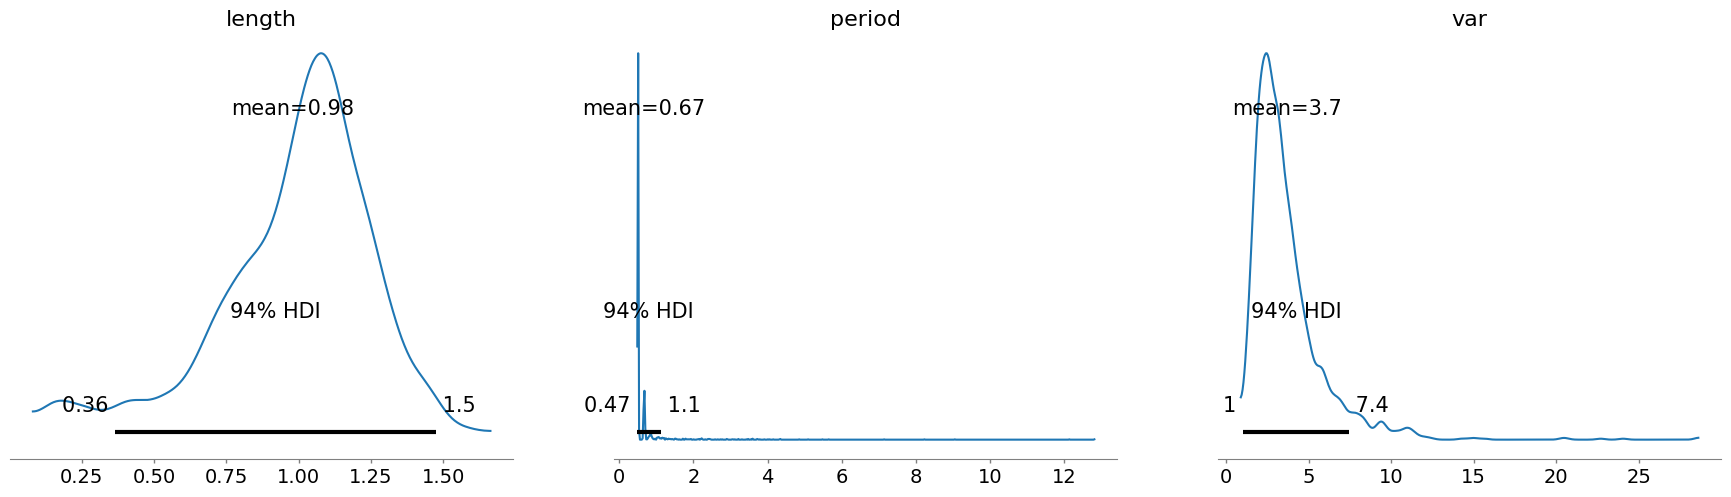
\includegraphics[width=1\textwidth]{./figures/nuts_post.png}
  \caption{
    Posterior samples of the parameters of the model.
  }
  \label{gp:nuts:post}
\end{figure}

\begin{figure}[htbp]
  \centering
  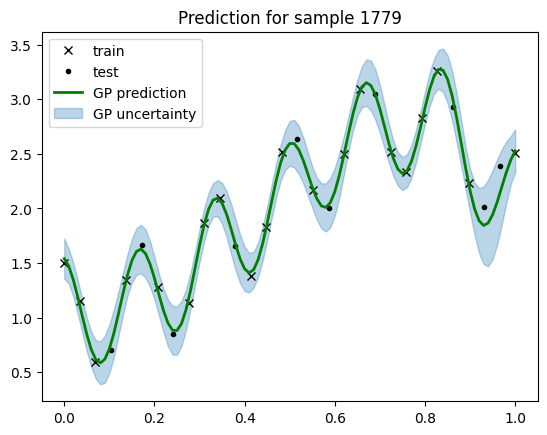
\includegraphics[width=0.6\textwidth]{./figures/nuts_pred.png}
  \caption{
    Random prediction using NUTS.
  }
  \label{gp:nuts:pred}
\end{figure}
\begin{figure}[htbp]
  \centering
  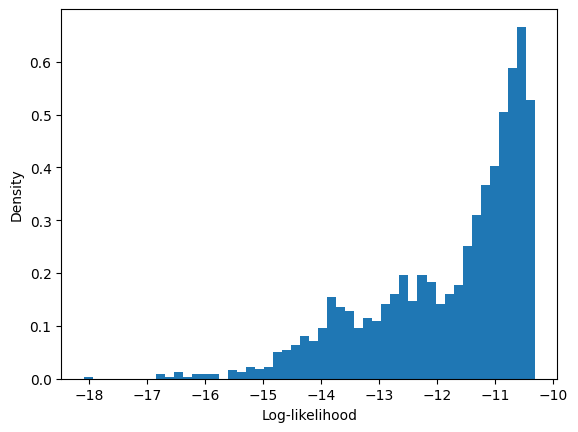
\includegraphics[width=0.6\textwidth]{./figures/nuts_ll.png}
  \caption{
    Distribution of log-likelihoods of test data
    from posterior samples using NUTS.
  }
  \label{gp:nuts:ll}
\end{figure}

For computing the posterior log-likelihoods,
we used the following equation
\begin{align*}
  \tp{y} \left( \epsilon I + K(X) \right)^{-1} y
  + \log{\text{det}| \epsilon I + K(X) |}
  + n \log{\sqrt{2 \pi}}
\intertext{where $n$ is the number of elements in $y$.}
\end{align*}

\subsubsection{Comparing MAP and NUTS}
For comparing the two methods,
we ran 20 iterations of each, with the same hyperparameters
as described before, except for NUTS we only used a single chain
to speed it up.

The log-likelihoods of the two methods is shown in~\cref{gp:map_nuts_ll}.
The mean and variance of the log-likelihoods are shown in~\cref{gp:map_nuts_ll_mean_var}.
From the comparison we see that NUTS performs slightly better on average,
but is also less consistent with a few poor model parameters.
Additionally, sampling with NUTS is much slower that training with MAP,
and so for this problem the MAP method worked best.

\begin{table}[H]
  \centering
  \begin{tabular}{lll}
    \toprule
    Method & Mean  & Variance \\
    \midrule
    MAP    & -9.93 & 9.57     \\
    NUTS   & -9.73 & 15.60    \\
    \bottomrule
  \end{tabular}  
  \caption{
    Mean and variance of log-likelihoods using MAP and NUTS.
  }
  \label{gp:map_nuts_ll_mean_var}
\end{table}

\begin{figure}[htbp]
  \centering
  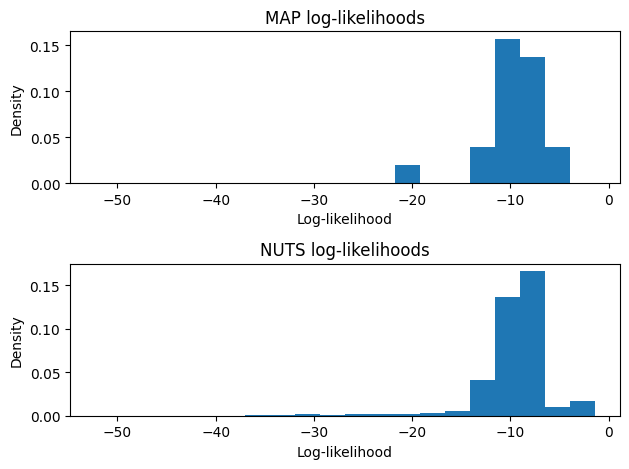
\includegraphics[width=0.6\textwidth]{./figures/map_nuts_ll.png}
  \caption{
    Comparing log-likelihoods when using MAP and NUTS.
  }
  \label{gp:map_nuts_ll}
\end{figure}

\subsection{Learning with Integral Constraints}

We write the constraint $\hat{q}$ in matrix form:

\begin{align*}
  \hat{q} = \sum_{i=1}^\ell w_i f(x_i) = {w} f
\end{align*}
where $w = \begin{bmatrix} w_1, \ldots, w_\ell \end{bmatrix}$
and $f = \tp{\begin{bmatrix} f(x_1), \ldots, f(x_\ell) \end{bmatrix}}$.
%
Writing the joint distribution of $(\hat{q}, f)$ as a matrix
and facotring out $f$ we get
\begin{align*}
  (\hat{q}, f)
  = \left[ \begin{array}{c} \hat{q} \\ \hline f \end{array} \right]
  = \left[ \begin{array}{c} w \\ \hline I \end{array} \right] f
  = Q f
\end{align*}
with $Q = \left[ \begin{array}{c} w \\ \hline I \end{array} \right]$.

As $f \sim \mathcal{GP}(0, k(\cdot, \cdot))$, then we must by definition have
$f | X \sim \mathcal{N}\left( 0, K(X) \right)$
and as multivariate normal distributions are closed under linear transformations
we therefore have
\begin{align*}
  (\hat{q}, f) | X
  = Q f | X
  \sim \mathcal{N}\left( 0, Q K(X) \tp{Q} \right).
\end{align*}

Letting ${\Sigma} = Q K(X) \tp{Q}$, we partition ${\Sigma}$
into four blocks
\begin{align*}
  {\Sigma} &=
  \left[
    \begin{array}{c|c}
      \Sigma_{1 1} & \Sigma_{1 2} \\
      \hline
      \Sigma_{2 1} & \Sigma_{2 2} \\
    \end{array}
  \right]
  \intertext{
    where
  }
  \Sigma_{1 1} = w K(X) \tp{w},
  \quad
  \Sigma_{1 2} &= w K(X),
  \quad
  \Sigma_{2 1} = K(X) \tp{w},
  \quad
  \Sigma_{2 2} = K(X).
\end{align*}
We then have that the conditional
$f | X, \hat{q} \sim \mathcal{N}(\mu_{2|1}, \Sigma_{2|1})$, where
\begin{align*}
  \mu_{2|1} = \Sigma_{2 1} \Sigma_{1 1}^{-1} \hat{q},
  \quad
  \Sigma_{2|1} = \Sigma_{2 2} - \Sigma_{2 1} \Sigma_{1 1}^{-1} \tp{\Sigma_{2 1}}
\end{align*}


To determine whether $\Sigma_{2|1}$ is full rank, we can check if $\Sigma_{2 | 1}$
has a trivial null space. This is equivalent to proving that there exists no
vector $v \ne \overrightarrow{0}$ such that $\Sigma_{2 | 1} v = \overrightarrow{0}$, since the existance of such a vector
implies that $v$ is contained in the null space of $\Sigma_{2 | 1}$ and thus is not full rank.
We prove that it is not full rank by contradiction. We let $v=\tp{w}$ since
$w$ was the weighting for our integral constraint (a linear operator that imposed a
constraint on our distribution) and $w$ will never be $\overrightarrow{0}$ by construction. We then have
\begin{align}
  \Sigma_{2|1} \tp{w}
  &= \left(K(X) - K(X) \tp{w} (wK(X)\tp{w})^{-1} \tp{\left(K(X)\tp{w}\right)}\right) \tp{w} \\
  &= K(X)\tp{w} - K(X) \tp{w} (wK(X)\tp{w})^{-1} \tp{\left(K(X)\tp{w}\right)} \tp{w} \\
  &= K(X)\tp{w} - K(X) \tp{w} (wK(X)\tp{w})^{-1} (w\tp{K(X)} \tp{w}) \\
  \intertext{We know that a quadratic form is equal to its transpose:}
  &= K(X)\tp{w} - K(X) \tp{w} (wK(X)\tp{w})^{-1} (wK(X) \tp{w}) \\
  &= K(X)\tp{w} - K(X) \tp{w}\\
  &= \overrightarrow{0}\quad \rightarrow \leftarrow
\end{align}
We have shown by contradiction that $\Sigma_{2|1}$ will never be full rank since $\tp{w}$ will 
always be in the null space of $\Sigma_{2|1}$. 
